\chapter{Cloud}
Cloud came out as a business model, not as a technlogy.
It was needed to handle peak of requests and to allow scalability, without oversizing Infrastructures.
\note{e.g. Amazon needs to handle way more requests on Christmas than on a normal day.}
So, Cloud was a mean to reduce the cost of the ICT infrastructure.

\textbf{Resource pooling} is the key concept of Cloud. It means that the services are provided to users using a multi-tenant model, with physical and virtual resources being dynamically allocated and deallocated according to the demand.\\
Cloud was needed also to provide rapid elasticity, meaning that capabilities may be elastically provisioned and released, in some cases automatically, to scale rapidly outward and inward commensurate with demand. To the customer it means that the capabilities available for provisioning often appear to be unlimited and can be appropriated in any quantity at any time.

Benefits of Cloud:
\begin{itemize}
   \item \textbf{Business agility}
   \begin{itemize}
      \item Quick resource provisioning
      \item Facilitates innovation
      \item Reduces time to market
   \end{itemize}
   \item \textbf{Reduces IT costs}
   \begin{itemize}
      \item Reduces up-front capital expenditure (CAPEX)
      \item Improves resource utilization
      \item Reduces operational expenditure (OPEX)
   \end{itemize}
   \item \textbf{High availability}
   \begin{itemize}
      \item Ensure resource availability based on customer's requirements
      \note{In RAI, prof. Cisternino experienced people complaining because their servers' CPUs were running at 98\% of their capability, and they wanted to exploit also the remaining 2\%, because ``they paid for it''.}
      \item Enables fault tolerance
      \note{Recall active-active, active-passive, etc. configurations.}
   \end{itemize}
   \item \textbf{Business continuity}
   \item \textbf{Flexible Scaling}
   \item \textbf{Flexibility of Access}
   \item \textbf{Application Dev and Testing}
   \item \textbf{Simplified infrastructure management}
   \item \textbf{Increased collaboration}
   \item \textbf{Masked complexity}
\end{itemize}
Cloud has the magic power of decoupling the software from the hardware.

Disadvantages of Cloud:
\begin{itemize}
   \item Vendor lock-in
   \item Privacy
   \item Your software depends on someone else
   \item Legislation is complicated
   \note{In EU public administration data, must be stored in the EU.}
   \item \dots TODO
\end{itemize}

\section{Cloud Service Models}
\begin{itemize}
   \item \textbf{IaaS} (Infrastructure as a Service)
   \begin{itemize}
      \item Provides virtualized computing resources over the Internet
      \item Examples: Amazon EC2, Google Compute Engine, Microsoft Azure
   \end{itemize}
   \item \textbf{PaaS} (Platform as a Service)
   \begin{itemize}
      \item Provides a platform allowing customers to develop, run, and manage applications without the complexity of building and maintaining the infrastructure
      \item Examples: Google App Engine, Microsoft Azure, Heroku
   \end{itemize}
   \item \textbf{SaaS} (Software as a Service)
   \begin{itemize}
      \item Provides software applications over the Internet
      \item Examples: Google Apps, Microsoft Office 365, Salesforce
   \end{itemize}
\end{itemize}

\section{Cloud Deployment Models}
\begin{itemize}
   \item \textbf{Public Cloud}
   \begin{itemize}
      \item Owned and operated by third-party cloud service providers
      \item Deliver computing resources over the Internet
      \item Examples: Amazon Web Services (AWS), Microsoft Azure, Google Cloud Platform
   \end{itemize}
   \note{It does \textbf{not} mean that the data is public. It means that the cloud services are accessible to the public.}
   \item \textbf{Private Cloud}
   \begin{itemize}
      \item Operated solely for a single organization
      \item Managed by the organization or a third party
      \item \textit{On-premise} or \textit{off-premise}
   \end{itemize}
   \note{It does \textbf{not} mean that the data is private. It means that the cloud services are accessible only to the organization e.g. \textit{UniPi}.}
   \item \textbf{Hybrid Cloud}
   \begin{itemize}
      \item Composition of two or more clouds (private, community, or public) that remain unique entities but are bound together, and resources may be moved from one cloud to another (with some performance cost obviously) 
      \item By standardized or proprietary technology that enables data and application portability
   \end{itemize}
   \item \textbf{Community Cloud}
   \begin{itemize}
      \item Shared infrastructure for specific community
      \item Managed by organizations or third party
      \item On-premises or off-premises
   \end{itemize}
\end{itemize}

\section{Control Layer}
The control layer is responsible for managing the resources and the allocation of the resources to the virtual machines.

\begin{definition}[Control Layer]
   ``The control layer is important because it's the way pool the resources set and see all the resources in a coherent way so it's a sort of a software layer that hides the differences and gives you primitives (such as ``I need a VM, I don't care where, but I need one'').''
\end{definition}


Note that you cannot allocate more virtual cores than the physical ones ---same applies to memory---, but you can allocate smaller pieces so you can create a resource pooling of resources that can be taken partially (assuming that they can run on a single node), but making you perceive it as a pool of resources.

Layers above the control layer have no clue where workloads are running, they just know that they do so somewhere, it is completely up to the control layer to manage where and how. 
\nl

The steps towards provisioning a resource are three
\begin{enumerate}
   \item \textbf{Resource Discovery}
   \item \textbf{Resource Pooling}
   \item \textbf{Resource Provisioning}
\end{enumerate}

A key component in the control layer is a Unified Manager software, which handles, by means of APIs, the tools associated to
\begin{itemize}
   \item Compute System management
   \item Fabric management
   \item Storage System management
\end{itemize}

\subsection{Resource Discovery}
The control layer enables \textbf{unified manager} to learn about resources that are available for service deployment
Provides visibility to each resource
Enables to manage cloud infrastructure resources centrally


\subsection{Resource Pooling and Provisioning}
A unified manager at control layer allows to categorize in \textbf{grading pools} resources and identity pools based on predefined criteria.
This helps creating variety of services decoupled from the actual hardware where they will run, but still providing choices to consumers on the type ---and amount--- of hardware they get (e.g. ``0.5TB Flash, 4TB SATA, 1TB FC'').
Multiple grade levels (e.g. ``Gold'', ``Silver'', ``Bronze'') may be defined for each type of pool, where costs/prices of resource pools differ depending on grade level.
\nl

\framedt{Resource provisioning starts when a user requests a service.}
{
   When I create a VM, i can choose the template (e.g. ``Windows 2016'', ``Ubuntu 18.04''), hardware, extensions, and lastly I will be asked to select a Host.
   At that point the system polls the control layer to see which hosts are available and which are not, and then rank them.
   Then I'll be asked for the chosen host the estimated workload on CPU (percentage), memory and disk.
   Set the host, the control software provides information regarding networking.
}

Lastly, it is important to recall that \textbf{Resource monitoring} is fundamental to keep track of the resources used and to prevent over-provisioning.

\subsection{Control Software demo}
   Prof. Cisternino demonstrated a Control Software he uses for the UniPi Cloud, where he can see the resources available and the resources allocated to the VMs.

   \begin{paracol}{2}
      \colfill
      In the ``VM and Services'' view, the software allows to see the different Clouds associated to Polo 1, Polo 2, etc. and the resources allocated to each of them.\\
      There is also another inner view to check VM networks and the actual hosts where the VMs are running.
      \colfill
      \switchcolumn
      \begin{figure}[htbp]
         \centering
         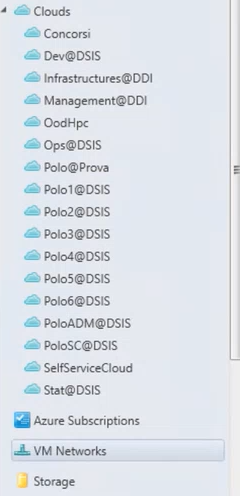
\includegraphics[width=0.45\columnwidth]{images/Control_VMandServices.png}
         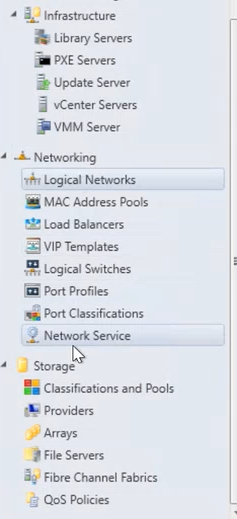
\includegraphics[width=0.45\columnwidth]{images/Control_FabricView.png}
         \caption{VM and Services view}
      \end{figure}
   \end{paracol}

   He may even open a Powershell terminal on a VM.

   \ul{This software allows him to manage about 1400 VMs.}
\section{Service Layer/Service Orchestration Layer}

\begin{definition}[Cloud Service]
   \label{def:cloudservice}
   IT resources that are packaged by the service providers and are offered to the consumers
\end{definition}
This means that deploying a service, does not mean simply deploying a VM, but a bunch of them, and also configuring it, installing software, etc. 

\textbf{Service Layer} enables defining services in a service catalog, and provides a self-service portal for users to request services (enables on-demand and self-provisioning).
\note{Essentially, the catalog is the DB while the cloud portal is the web interface for it.}

\subsection{Service Orchestration Layer}
\textbf{Service Orchestration layer} implements the process of integrating services to support the automation of business processes:
\ul{actuates the policies and the requests automatically from the user}.

\begin{figure}[htbp]
   \centering
   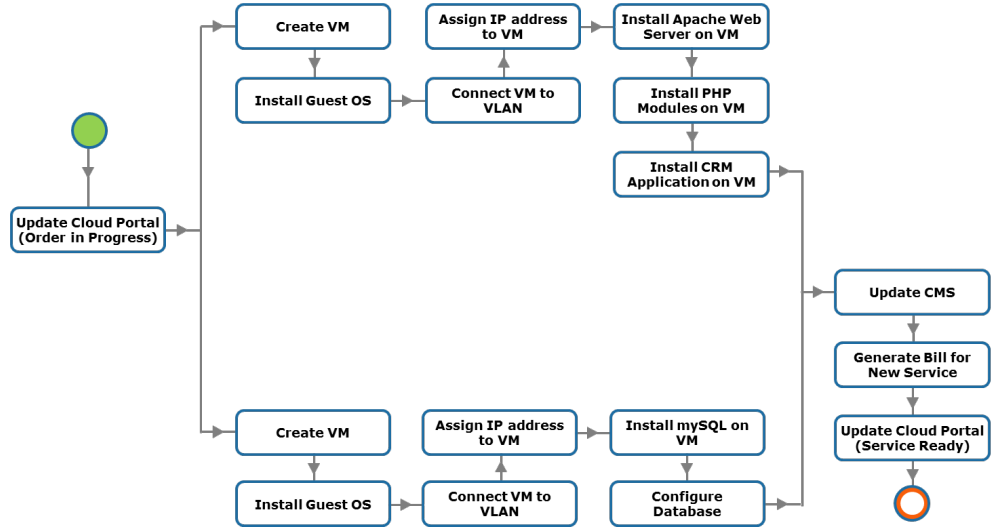
\includegraphics[width=0.45\columnwidth]{images/serviceorchestration1.png}
   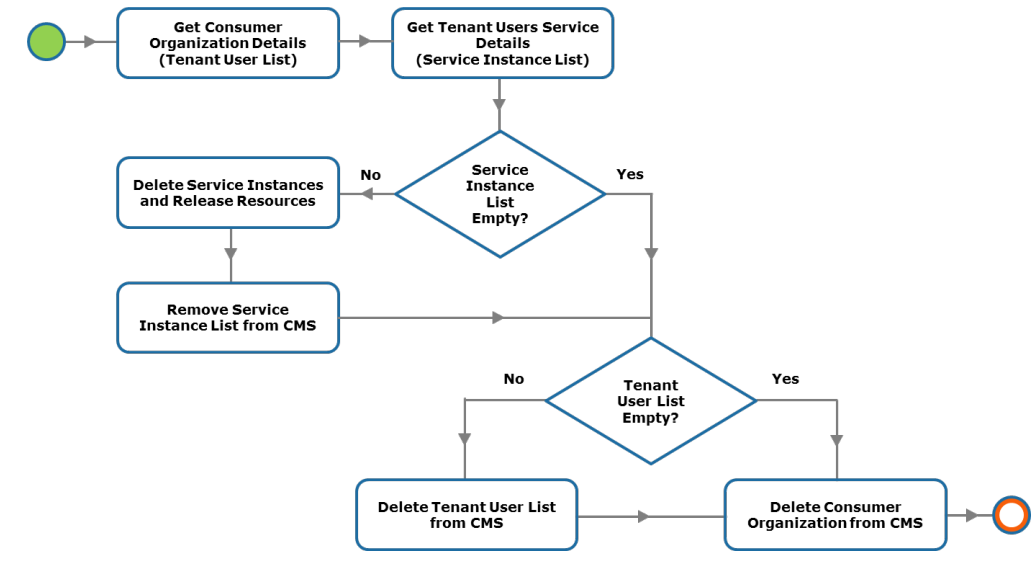
\includegraphics[width=0.45\columnwidth]{images/serviceorchestration2.png}
   \caption{Service orchestration layer use cases. On the left, provisioning a CRM application, while on the right a tenant removal}
   \label{fig:serviceorchestration}
\end{figure}
\begin{definition}[Tenant] A tenant is a user of the cloud, and the cloud provider must ensure that the tenant is isolated from the others. This is done by means of \textbf{multi-tenancy}.
\end{definition}
\note{UniPi\st{.it} is a tenant for Microsoft Azure.}
\nl

\subsection{Deeper into Services}
\begin{paracol}{2}

   We may generalize the \ul{\textbf{lifecycle} of a service} as it is depicted in Figure \ref{fig:servicelifecycle}, split in 4 main phases:
   \ns
   \begin{enumerate}
      \item \textbf{Planning}
      \begin{enumerate}
         \item Assessing service requirements
         \item Developing service enablement roadmap
         \item Establishing billing policy
      \end{enumerate}
      \item \textbf{Creation}
      \begin{enumerate}[ref=\theenumi{}.\roman*]
         \item Defining service template
         \item Creating orchestration workflow
         \item Defining service offering
         \item Creating service contract\label{enum:SLA}
      \end{enumerate}
   \end{enumerate}
   \switchcolumn
   \colfill
   \begin{enumerate}[start=3]
      \item \textbf{Operation}
      \begin{enumerate}
         \item Discovering service assets
         \item Managing service operations
      \end{enumerate}
      \item \textbf{Termination}
      \begin{enumerate}
         \item Natural termination by contract agreement
         \item Initiated termination by a provider or a consumer          
      \end{enumerate}
   \end{enumerate}
   \colfill
\end{paracol}
\begin{figure}[htbp]
   \centering
   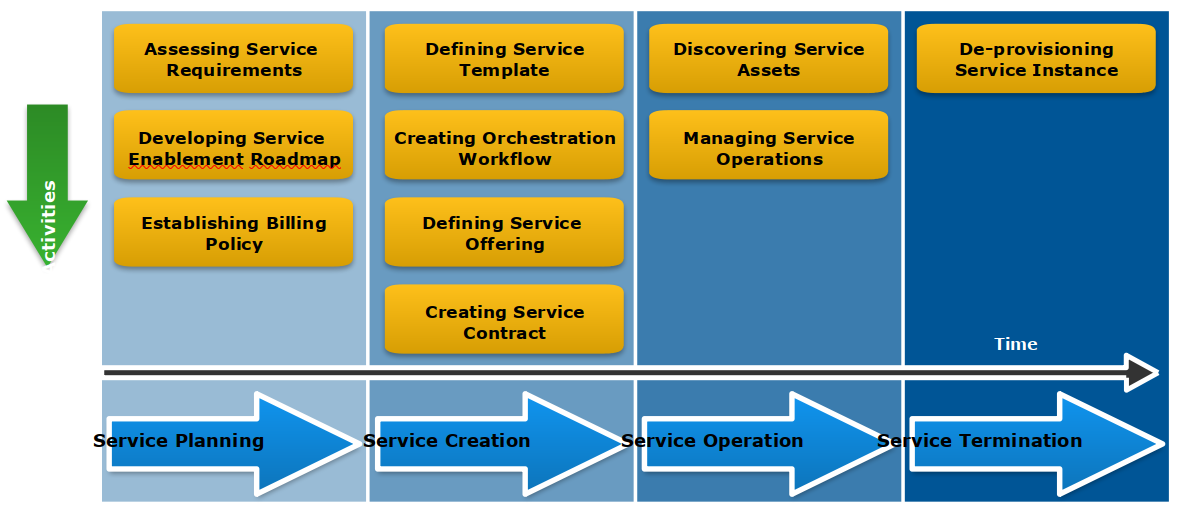
\includegraphics{images/servicelifecycle.png}
   \caption{Service Lifecycle schema}
   \label{fig:servicelifecycle}
\end{figure}

Having defined what a Service is \ref{def:cloudservice}, we can now define the \textbf{Service Layer} as the layer that provides the services to the users.

Step \ref{enum:SLA} refers ---also--- to the Service Level Agreement, which basically is the legalese version of the set of resources that we are allocating for a user.\\
Aside from the SLA, other parameters are discussed such as pricing, termination of service and possibly other configuration aspects.

\framedt{
   ``If you are smart enough you may trick the user''
}{
   Amazon tricked a user by establishing a SLA that said that the user would have a 99.999\% uptime, but they considered uptime even when the service was both not available and \textit{not} requested by the user.
}

\section{Business Continuity}
\begin{definition}[Business Continuity]
   The capability of an organization to continue delivery of products or services at acceptable predefined levels following a disruptive incident.

   \emph{\dots or \dots}
   
   BC entails preparing for, responding to, and recovering from service outage that adversely affects business operations
\end{definition}

\textbf{SPOF}s may occur at component level, or at site or data center level.\\
The key to avoid SPOFs is to have redundancy, which may be achieved by means of \textbf{replication} or \textbf{backup}s (more on this later).
\nl

\begin{definition}[Compute Clustering]
   A technique where at least two compute systems (or nodes) work together and are viewed as a single compute system to provide high availability and load balancing. 

\end{definition}
Enables service failover in the event of compute system failure to another system to minimize or avoid any service outage.\\
The implementation may be \textit{active-active} or \textit{active-passive}.

\subsection{Data Protection}
A \textbf{backup} is not simply a copy of the current data to be used in case a disk fails. In case a ransomware attack occurs, the copy will be encrypted as well, or even more trivially, if a service has a bug and it corrupts data, also the copy would contain bad data.\\
``\ul{Backup must allow to travel back in time.}''

The two critical terms are \textit{Recovery Time Objective} (\texttt{RTO}) and  \textit{Recovery Point Objective} (\texttt{RPO})\footnote{Point in time}.
They refer to the time it takes to recover from a disaster and the amount of data that can be lost respectively.

Backups are typically done incrementally, meaning that starting from a full backup, then only differences are stored.
However, saving storage in this way leads to a more complex recovery process, as all the incremental backups must be applied to the full backup to recover the data, possibly considerably increasing the RTO.\\
To overcome the issue, a full backup is done every now and then e.g. a week is common practice, and incremental daily backups are done until the next full backup.\\
This fixes the RPO to 1 day, while the RTO still may vary depending on bandwidth, storage speed, and most importantly size and amount changes throughout time; typically it is days (?) or hours.